\documentclass[a4paper,12pt]{elsarticle}
\usepackage[a4paper]{geometry}
\usepackage[cm]{fullpage}
\usepackage{amsthm,amsmath,amssymb}
\usepackage{graphicx}
\usepackage{url}
\usepackage{natbib}
\usepackage{hyperref}

\numberwithin{equation}{section}
\theoremstyle{plain}
\newtheorem{theorem}{Theorem}[section]
\newtheorem{lemma}[theorem]{Lemma}
\newtheorem{proposition}[theorem]{Proposition}
\newtheorem{cor}[theorem]{Corollary}
\theoremstyle{definition}
\newtheorem{defi}[theorem]{Definition}
\newtheorem{example}[theorem]{Example}
\theoremstyle{remark}
\newtheorem{remark}[theorem]{Remark}
\numberwithin{equation}{section}

\newcommand{\Rd}{\mathbb R^d}
\newcommand{\spc}{\mathbb R}
\newcommand{\spctim}{\spc \times [0,\infty)}
\newcommand{\R}{\mathbb R}
\newcommand{\1}{\mathbf 1}
\newcommand{\pr}{\mathbf P}
\newcommand{\ex}{\mathbf E}
\newcommand{\del}{\partial}


\begin{document}

\begin{frontmatter}

\title{Variable Order Fractional Fokker-Planck Equations derived from 
Continuous Time Random Walks}
\author[UNSW]{Peter Straka}
\ead{p.straka@unsw.edu.au}
\address[UNSW]{School of Mathematics \& Statistics, UNSW Sydney}


\begin{abstract}
We consider subdiffusive scaling limits of Continuous Time Random Walks (CTRWs),
in the case where the distribution of the waiting times and thus
the resulting memory kernel varies with the location in space.  We first 
establish a 
one-to-one correspondence between CTRW limit processes and Langevin processes in 
space-time.  In this space-time representation, the evolution of the waiting 
times is readily governed by varying their L\'evy measure and drift in space. 
In the case of fractional diffusion and tempered fractional diffusion, this 
can be expressed via a varying fractional parameter $\beta(x) \in (0,1)$ and/or 
a varying tempering parameter $\theta(x) \ge 0$, as well as a varying 
``temporal drift'' parameter $d(x) \ge 0$. 
We then use a result from the mathematics literature which identifies the 
probability distributions of a CTRW limit process with the unique solution 
of a Fokker-Planck equation with memory.  We then focus on the situation where the CTRW 
dynamics are locally fractional with parameter $\beta(x)$.  We rigorously derive 
the variable order fractional Fokker-Planck equation (FFPE) from the CTRW limit.  This equation 
displays a unique temporal scaling behaviour: given a time scale parameter $T_0$, the factor $T_0^{-\beta(x)}$ 
enters in both the drift and diffusivity coefficients of the Fokker-Planck operator.  
We present Monte Carlo simulations which show that solutions to the variable 
order FFPE are consistent at different time scales. 
\end{abstract}

% Cover Letter

% Dear Editorial Office,

% Please find attached a manuscript titled "Variable Order Fractional Fokker-Planck Equations derived from Continuous Time Random Walks" which I would like to submit for your consideration as an original research article to be published in Physica A. 

% Anomalous diffusion has been a hot topic in statistical physics in the past two decades, due to its relevance in biophysics, hydrology etc. as well as due to the rich and applicable theory provided by the fractional Fokker-Planck equation (FFPE). Whilst media with varying fractionality have attracted interest and numeric methods for solving variable-order FFPEs have been developed, a rigorous derivation of variable-order FFPEs from Continuous Time Random Walk processes is not available in the literature. This paper provides this derivation, and along the way uncovers some novel scaling behaviour of the variable order FFPE.

% The main tools used in the derivation come from the mathematical literature on Markov process scaling limits and lead to interesting new physics which are of interest to the anomalous diffusion community as well as the statistical physics audience in general.  Hence Physica A is a highly suitable journal for this manuscript. 

% Highlights: 
% - For the first time, a variable order Fractional Fokker-Planck equation is derived from scaling limits of Continuous Time Random Walks
% - The novel approach via bivariate Langevin Processes identifies all possible memory kernels as tail functions of Levy measures
% - The variable order fractional Fokker-Planck equation displays novel scaling behaviour, where drift and diffusivity depend on the time-scale
% - A general approach is given which constructs approximating sequences of Continuous Time Random Walks to solutions of a broad class of Fokker-Planck equations with memory


\begin{keyword}
Anomalous Diffusion \sep Continuous Time Random Walk \sep Fractional Derivative \sep Variable Order \sep stochastic process limit \sep L\'evy process \sep Fokker-Planck
\MSC[2010] 60F17 \sep  60G22
\end{keyword}

\end{frontmatter}


\section{Introduction}

Subdiffusive processes are characterized by a sublinearly growing mean squared
displacement proportional to $t^\beta$, $0 < \beta < 1$, and have been reported
in many experimental systems
\cite{Metzler2000,TMT04,Santamaria2006a,Banks2005,Regner2013}.
For a majority of these systems, long rests of a walker are thought to be the
main mechanism causing subdiffusion, and Continuous Time Random Walks (CTRWs)
with heavy-tailed waiting times effectively capture this phenomenon
\cite{Scher1975,BG1990,Metzler2000}.  CTRWs have become a widely used model,
particularly because scaling limits of their probability distributions can be
modelled by fractional differential equations and Fokker-Planck equations
\cite{BMK00,Baeumer2001,HLS10PRL,Hahn11} which can be extended tractably to
model particle reactions \cite{Langlands2008d,Angstmann2013} and nonlinear
interaction effects \cite{StrakaFedotov14}.

In the majority of the literature on CTRWs and FFPEs (fractional Fokker-Planck
equations), the
fractional parameter $0 < \beta < 1$ is treated as a global constant.  The
situation where $\beta$ varies in space, however, is of interest in physics,
since the strength of a trapping effect may vary throughout a disordered
medium
\cite{Chechkin2005a,Korabel2010,Stickler2011,Fedotov2012,StrakaFedotov14}.
The experiments in \cite{Wong04} find that for the diffusion of a bead in
F-actin networks, the fractional parameter depends solely on the ratio of
bead size to mesh width, and hence a physical system with continuously varying
fractional parameter could be constructed.

There are various works in the computational literature that consider ``variable
order'' fractional subdiffusion equations (see e.g.\ \cite{Chen2010,Sun2009} and
the references therein). Candidate fractional differential equations of
variable order for a spatially varying subdiffusive system are:
\begin{align}
\label{eq:wrong1}
  &\cite[Eq.(8)]{Sun2009}:
  &
  D_t^{\beta(x)} u(x,t) &= K \frac{\partial^2 u(x,t)}{\partial x^2}
  \\
  \label{eq:wrong2}
  &\cite[Eq.(1.2)]{Chen2010}:
  &
  \frac{\partial u(x,t)}{\partial t} &= K {_0 D_t^{1-\beta(x)}}
  \frac{\partial^2 u(x,t)}{\partial x^2} + f(x,t)
\end{align}
In \eqref{eq:wrong1}, the fractional temporal derivative is of Caputo type,
whereas in \eqref{eq:wrong2}, it is of Riemann-Liouville type.
We note the following issues in the applicability of these two prototypes:
\begin{itemize}
  \item
  Both equations appear to be dimensionally inconsistent: an application of the
  fractional derivative of order $\beta$ is dimensionally equivalent to a
  division by Time$^{\beta}$. One side of the equation has dimensions
  independent of $x$, whereas the other side does depend on $x$.  A
  non-dimensional interpretation of the differential equation seems to be
  necessary, but it is unclear how time scale parameters enter into the
  equation, or how dynamics are related at two different time scales.
  \item
  For the two equations to be equivalent, the fractional integral needs to
  commute with the diffusion coefficient $K$ and the drift coefficient $b$,
  if present.  Unless these coefficients are constant, this is not the case,
  and the question arises which one to choose.
  \item
  Neither equation has been derived from a CTRW scaling limit. Such a derivation
  would be useful, since it would e.g.\ guarantee positivity of solutions,
  provide means to compare probability densities with Monte Carlo simulations,
  and allow extensions for chemical reactions or other particle interaction.
\end{itemize}

In this article, we resolve the issues above.  We provide a general approach
which represents CTRW scaling limits as Langevin processes in space-time
$\spctim$.  In the space-time setting, spatially varying parameters for the
waiting time distribution are mathematically tractable and dimensionally
coherent.  The general form of the FFPE (Fractional Fokker-Planck Equation)
governing a CTRW limit becomes
\begin{align}
\frac{\del P(y,t)}{\del t} = \mathcal L^*(y,t) \left[ \frac{\partial}{\partial t}
\int_0^t P(y,t-s) V(y,s)\,ds \right] + h(y,t),
\end{align}
where $\mathcal L^*(y,t)$ is a Fokker-Planck operator with space- and
time-dependent drift and diffusivity, and
where the $y$-dependent memory kernel $V(y,s)$ admits an interesting 
interpretation
based on renewal theory.  In particular, if the dynamics are locally fractional
with parameter $\beta(y)$, then the governing equation changes dependent on the 
time scale $T_0$, and the FFPE is
\begin{align} \label{eq:VOFFPE}
\frac{\del P(y,t)}{\del t}
= \mathcal L^*(y,t) \left[ T_0^{-\beta(y)} {_0 D}_t^{1-\beta(y)} P(y,t) \right] + h(y,t),
\end{align}
where ${_0 D}_t^{1-\beta(y)}$ is the order $1-\beta(y)$ Riemann-Liouville
fractional derivative.  This equation extends \eqref{eq:wrong2} to
space- and time-dependent drift and diffusivity and allows for a switch
between time scales.


Section 2 describes the underlying dynamics in space-time, where the first
component tracks the location of a particle and the second component the
physical time that has passed.  Scaling limits are identified as bivariate
Langevin processes which uniquely correspond to CTRW limits.
In Section 3 we utilize a result from the mathematics literature that links CTRW 
limits with fractional Fokker-Planck equations.
In Section 4 we show that the variable-order FFPE \eqref{eq:VOFFPE} is consistent, by  calculating matching solutions at different time scales via a Monte-Carlo simulation of CTRW trajectories.


\section{The space-time setting}

\subsection{CTRWs are space-time Markov Chains}

The trajectory of a CTRW can be reduced to a series of points in
space-time, without loss of information: If $t_1, t_2, \ldots$
denote the jump times of a CTRW and $x_1, x_2, \ldots$ the locations
of the end points of the jumps, then the location of the CTRW at time
$t$ is
\begin{align} \label{eq:CTRW-trajectory}
X^{(c)}_t = x_k \text{ for } k \ge 0 \text{ such that }
t_k \le t < t_{k+1}.
\end{align}
We write $c$ for a scaling parameter, as will be detailed below.
Moreover, write $t_0$ for the starting time and $x_0$ for the starting
location. Then the pair sequence
$(t_0, x_0), (t_1, x_1), (t_2, x_2), \ldots$
must define a Markov chain in space-time $\spctim$,
by the CTRW assumption that the $k+1$-th waiting time $t_{k+1} - t_k$
and the $k+1$-th jump $x_{k+1} - x_k$ are both independent of the past
$(t_0, x_0), \ldots, (t_{k-1}, x_{k-1})$ given the current $(t_k, x_k)$.

The distribution of the Markov chain $(t_k, x_k)$ is thus uniquely
determined by the initial location $(x_0, t_0)$ in space-time,
and a probability kernel on space-time
\begin{align} \label{eq:STJK}
K^{(c)}(y,w | x,s)
\end{align}
denoting the probability distribution of the next jump 
$y = x_{k+1} - x_k$ after the next waiting time
$w = t_{k+1} - t_k$, conditional on $(x_k, t_k) = (x,s)$.
As an example, let $(t_0, x_0) = (0,0)$ and
\begin{align} \label{eq:STJK-example}
K^{(c)}(y,w | x,s) = \left[\frac{1}{2} \delta_{+\chi}(y) + \frac{1}{2} \delta_{-\chi}(y)\right] \beta(x) (1+w/\tau)^{-1-\beta(x)} \, dw,
\quad w > 0, \quad \beta(x) \in (0,1).
\end{align}
Then \eqref{eq:STJK-example} defines a CTRW with Pareto waiting times at scale
$\tau$ and jumps $\pm \chi$ with equal probability $1/2$.  The tail parameter 
$\beta$ varies as a function $\beta(x)$ in space. 


We will view $c > 0$ as a ``master'' scaling parameter, and we let
$\tau = 1/c$ for the temporal scale and $\chi = c^{-1/2}$ for the
spatial scale.
Thus for every $c$ we have defined a Markov chain on $\spctim$, which
in turn defines a CTRW at scale $\chi$ in space and $\tau$ in time
via \eqref{eq:CTRW-trajectory}.
We are interested in the limiting CTRW process $c \to \infty$.


\subsection{The limiting space-time Langevin Process}

We seek to identify and characterize a class of possible limit processes
$(Y_u, Z_u)$ of the above Markov chains,
in the scaling limit as $c \to \infty$. As it turns out, this class of 
limiting stochastic processes are solutions to
Langevin equations in space-time (or solutions to stochastic differential
equations with L\'evy noise, or ``jump-diffusions'').
We characterize this class of Langevin processes in this section, and detail 
a construction of these processes via Poisson Random Measures.
Then in Section \ref{subsec:convergence}, we utilize results from the theory of
convergence of stochastic processes to give exact conditions of convergence
to these Langevin processes.

\paragraph{Poisson Random Measure}
The standard construction of L\'evy noise is via Poisson Random Measures
\cite{Applebaum}.  We describe an approach which is amenable to spatially 
varying coefficients. 
We first define the mean measure $M$ to be the Lebesgue measure on 
$(0,\infty) \times [0,\infty)$; the first component $(0,\infty)$ corresponds 
to the size of the jumps $w > 0$ of the temporal component $Z_u$, whereas $[0,\infty)$
corresponds to an auxiliary time, during which these jumps accumulate. 
Lebesgue measure is nothing but the surface measure, defined by the requirement 
that a rectangle $B = (a,b) \times (c,d) \subset (0,\infty) \times [0,\infty)$
have the measure $M(B) = (b-a)(d-c)$.  
A Poisson Random Measure with intensity measure $M$ is a random measure 
$N(dw, ds) = \sum_{r \in \mathcal R} \delta_{r}(dw, ds)$ where $\delta_r$ 
denotes a Dirac point measure at the point $r \in (0,\infty) \times [0,\infty)$
and $\mathcal R \subset (0,\infty) \times [0,\infty)$ is a random set of points 
such that the following two criteria hold: 
\begin{itemize}
  \item 
  For any bounded rectangle $B$, the cardinality of the set $\mathcal R \cap B$,
  i.e.\ the number of 
  points of $\mathcal R$ that lie in $B$, is Poisson distributed with mean 
  $M(B)$.
  \item
  The point counts in disjoint rectangles are independent. 
\end{itemize}

\paragraph{L\'evy measure}
The points in $\mathcal R$ are transformed in their first component according 
to the \emph{coefficient function} $F$.  For instance, if we let 
\begin{align} \label{eq:coefficient-F}
  F(w) = \left( \Gamma(1-\beta) w \right)^{-1/\beta}, \quad 0 < \beta < 1
\end{align}
then it is not difficult to confirm that the set of points 
$F(\mathcal R) := \{(F(w), s): (w,s) \in \mathcal R\}$ 
define a Poisson Random Measure on $(0,\infty) \times [0,\infty)$ with mean 
measure 
\begin{align}
  M_F((a,b) \times (c,d)) = \int_a^b \nu(w)\,dw \times (d-c),
\end{align}
where 
\begin{align} \label{eq:stable-levy-measure}
\nu(w) = \frac{\beta}{\Gamma(1-\beta)} \, w^{-1-\beta}, \quad w > 0, \quad 
0 < \beta < 1.
\end{align}
The density $\nu$ satisfies\footnote{$a \wedge b := \min\{a, b\}$}
\begin{align}
\label{eq:Levy-condition}
\int_{w > 0}(1 \wedge w) \nu(w)\,dw < \infty,  
\end{align}
and is hence called a \emph{L\'evy measure};
the points in $F(\mathcal R)$ are referred to as \emph{L\'evy noise}.
Finally, the L\'evy process $Z_u$ is constructed from L\'evy noise via 
\begin{align} \label{eq:summed-noise}
  Z_u = \int\limits_{0 \le s \le u} \int\limits_{w > 0} F(w) N(dw,ds)
  := \sum_{(w,s) \in \mathcal R:\, s \le u} F(w).
\end{align}
Note that condition \eqref{eq:Levy-condition} guarantees the convergence of the 
sum in \eqref{eq:summed-noise}. 
Increasing L\'evy processes are called subordinators in the mathematics
literature.  If $F$ is chosen as in \eqref{eq:coefficient-F}, then the above 
subordinator has stable marginals, i.e.\ its Laplace 
transforms are \cite{Bertoin04}
\begin{align}
  \langle \exp(-\lambda Z_u) \rangle = \exp(-u \lambda^\beta), \quad u \ge 0.
\end{align}
 


\paragraph{Tempered $\beta$-stable subordinator}
A tempered $\beta$-stable subordinator has a L\'evy measure of the form
\begin{align}
  \label{eq:tempered-stable-levy-measure}
  \nu(w) = \frac{\beta}{\Gamma(1-\beta)}\, w^{-1-\beta}\,e^{-\theta w}\,dw, 
  \quad w > 0, \quad 0 < \beta < 1, \quad \theta \ge 0. 
\end{align}
Here $\theta$ is called the tempering parameter. A positive $\theta$ decreases 
the occurrence of very large jumps $w$ of $Z_u$, and the mean of $Z_u$ becomes 
finite.  If instead of \eqref{eq:coefficient-F} we let 
\begin{align} \label{eq:general-F}
  F(w) = \inf\left\lbrace z > 0: \overline \nu(z) \le w \right\rbrace
\end{align}
where $\overline \nu(z) = \int_z^\infty \nu(w')\,dw'$ and $\nu$ is as in \eqref{eq:tempered-stable-levy-measure}, then 
\eqref{eq:summed-noise}
yields a tempered stable subordinator $Z_u$.

\paragraph{Varying noise}
We now assume that the coefficients $\beta$ and $\theta$ of the tempered 
$\beta$-stable subordinator are functions of $x$, the location in space. 
To this end, we make 
\eqref{eq:tempered-stable-levy-measure} space-dependent via
\begin{align}
  \label{eq:varying-tempered-stable-levy-measure}
  \nu(w | x) = \frac{\beta(x)}{\Gamma(1-\beta(x))}\, 
  w^{-1-\beta(x)}\,e^{-\theta(x) w}\,dw, 
  \quad w > 0, \quad 0 < \beta < 1, \quad \theta \ge 0, 
\end{align}
where we assume that $\beta(x) \in (0,1)$ and $\theta(x) \ge 0$ are  
functions of $x$.
We also make the coefficient function \eqref{eq:general-F} space-dependent via
\begin{align} \label{eq:varying-general-F}
  F(w|x) = \inf\left\lbrace z > 0: \overline \nu(z | x) \le w 
  \right\rbrace,
\end{align}
where $\overline \nu(z | x) = \int_z^\infty \nu(w'|x)\,dw'$.
Thus $Z_u$ is a tempered stable subordinator with parameters $\beta(x)$ and 
$\theta(x)$. 
We have now set up the necessary tools for the limiting Langevin 
dynamics $(Y_u, Z_u)$ in space-time.

\paragraph{Space-time Langevin Process}
The class of scaling limits $(Y_u, Z_u)$ which is suitable for our CTRW setting 
is given by the following type of Langevin process in $\spctim$: 
\begin{align} \label{eq:SDEY}
dY_u &= b(Y_{u-}, Z_{u-})\,du + a(Y_{u-}, Z_{u-})\, dW_u \\
\label{eq:SDEZ}
dZ_u &= d(Y_{u-})\,du + \int_{w > 0} F(w | Y_{u-}) \, N(dw, du).
\end{align}
Here $Y_u$ denotes location in space; $Z_u$ the corresponding (physical) time;
$u$ denotes auxiliary time, resulting from the rescaled number of CTRW steps;
$W_u$ is independent Gaussian noise; $b$ and $a$ are space- and time-dependent
spatial drift resp.\ diffusivity functions; $d \ge 0$ is a temporal drift coefficient function;
and $F$ is as in \eqref{eq:varying-general-F}.

The distinction between physical time $Z_u$ and auxiliary time $u$ is helpful
as it allows to maintain a coherent physical interpretation of the FFPE derived
in Section \ref{sec:FFPE}.  The coefficient functions $b$ and $a$ measure
length (resp.\ length squared) \emph{per unit auxiliary time}.  Similarly,
$d$ measures physical time per unit auxiliary time, and $F$ is physical
time-valued.
Equation \eqref{eq:SDEY} has already appeared in \cite{Weron2008}, where
it was assumed that $Z_u$ is a homogeneous $\beta$-stable subordinator (L\'evy
flight).
The inhomogeneous form of $Z_u$ in \eqref{eq:SDEZ} is key to the generalization
to CTRW scaling limits with spatially inhomogeneous waiting times.



\paragraph{Conditions on coefficient functions}
If the coefficient functions $a, b, d$ and $F$ satisfy certain local 
Lipschitz and growth conditions \cite[Chapter 6]{Applebaum}, then the bivariate
Langevin equation \eqref{eq:SDEY} -- \eqref{eq:SDEZ} has a unique stochastic 
process solution.  Specifying $F(w|x)$ to the form \eqref{eq:varying-general-F} which depends on 
$\beta(x)$ and $\theta(x)$, we can employ a result by \cite{Tsuchiya1992}, 
which states that the Lipschitz and growth conditions are 
satisfied if we assume that the functions $a$, $b$, $d$, $\beta$ and $\theta$ 
are bounded and continuously differentiable with bounded derivative.
See Section~\ref{subsec:Lip-gro} for details.


\subsection{Limit theorem for the Langevin equation}
\label{subsec:convergence}
\paragraph{Infinitesimal generator}
The limiting Langevin stochastic processes $(Y_u,Z_u)$ are (Feller-)\footnote{Feller processes assume that at any time $t$, their distribution depends continuously on the starting point, here $(x,s)$.} Markov
processes, and as such their distributions
are uniquely determined by their infinitesimal generator
\begin{align}
\mathcal A f(x,s) = \lim_{u \downarrow 0}
\left \langle f(Y_u, Z_u)\right \rangle_{(x,s)} / u, 
\quad f \in C_0(\spctim)
\end{align}
where $f$ is a generic function\footnote{From the Banach space
$C_0(\spctim)$ of continuous  functions on $\spctim$ which vanish at $\infty$},
and $\langle \, \rangle_{(x,s)}$ denotes the ensemble average over all
trajectories starting at $(x,s)$ \cite{Applebaum}. The domain of $\mathcal A$ contains the twice
continuously differentiable functions, and $\mathcal A$ has the following
form:
\begin{align} \label{eq:inf-gen}
\begin{split}
\mathcal A f(x,s)
&= b(x,s)\frac{\del }{\del x} f(x,s)
+\frac{1}{2} a(x,s) \frac{\del^2}{\del x^2} f(x,s)\\
&+ d(x) \frac{\partial}{\partial s} f(x,s)
+ \int_0^\infty \left[f(x,s+w)-f(x,s)
\right] \nu(w|x)\, dw
\end{split}
\end{align}
We note three assumptions that have gone into \eqref{eq:inf-gen}: 
\begin{itemize}
\item
As $Z_u$ is a scaling limit of sums of positive waiting times,
we may restrict $Z_u$ to be non-decreasing; this means that
$Z_u$ has no diffusive component (i.e.\ the second derivative only applies to 
the spatial variable), that $\nu(w|x) = 0$ for $w \le 0$
(only positive jumps), and $d(x) \ge 0$.
\item
We assume that $Y_u$ is continuous (does not jump),
and so the L\'evy noise only enters the temporal component $Z_u$.
\item
The distribution of waiting times is assumed to depend on space only and not
on the current time; hence $d(x)$ and $\nu(w|x)$ only depend on $x$ and not on $s$.
\end{itemize}

\paragraph{Conditions for stochastic process convergence}
Define the following continuous time Markov jump process $(Y^{(c)}_u, Z^{(c)}_u)$ on 
$\spctim$: at location $(x,s)$, wait an amount of time which is exponentially distributed with mean $1/c$. (This time is in ``auxiliary time'', and is not a CTRW waiting time!) Then jump to the location $(x+y, s+w)$, where the distribution of $(y,w)$ is determined by \eqref{eq:STJK}, and repeat. 

It then follows (see e.g.\ \cite[Proposition 17.2]{Kallenberg}) that 
$(Y^{(c)}_u, Z^{(c)}_u)$ has the infinitesimal generator
\begin{align} \label{eq:jump-process-generator}
\mathcal A^{(c)} f(x,s) = c \int [f(x+y, s+w) - f(x,s)] K^{(c)}(y,w | x,s)\,dy\,dw.
\end{align}
A key result is \cite[Theorem 17.25]{Kallenberg}, which says that we may characterize convergence as follows:\footnote{The convergence on the left side of \eqref{eq:generator-condition} is in the sense of stochastic processes with respect to the Skorokhod $J_1$ topology, see e.g.\ \cite{Whitt2010}. The right side must hold for all $f$ from the domain of $\mathcal A$, which is a dense subset of the function space $C_0(\spctim)$ of continuous real-valued functions defined on $\spctim$ which vanish at $\infty$).}
\begin{align} \label{eq:generator-condition}
\lim_{c \to \infty}(Y^{(c)}_u, Z^{(c)}_u) = (Y_u, Z_u)
\text{ if and only if }
\lim_{c \to \infty} \mathcal A^{(c)}f(x,s) = \mathcal A f(x,s), 
f \in {\rm Dom}(\mathcal A)
\end{align}
The two theorems below connect \eqref{eq:generator-condition} to the convergence of CTRWs: 

\begin{theorem} \label{theorem1}
The right side of \eqref{eq:generator-condition} holds if the following 
conditions all hold: 
\begin{align} \label{eq:cond1}
\lim_{\epsilon \downarrow 0} \lim_{c \to \infty}
c \iint\limits_{|y|< \epsilon,\,0<  w < \epsilon} y K^{(c)}(y,w | x,s)\,dy\,dw &= b(x,s)
\\ \label{eq:cond2}
\lim_{\epsilon \downarrow 0} \lim_{c \to \infty}
c \iint\limits_{|y|< \epsilon, \,0<w < \epsilon} y^2 K^{(c)}(y,w | x,s)\,dy\,dw &= a(x,s)
\\ \label{eq:cond3}
\lim_{\epsilon \downarrow 0} \lim_{c \to \infty}
c \iint\limits_{|y|< \epsilon, \,0<w < \epsilon} w K^{(c)}(y,w | x,s)\,dy\,dw &= d(x)
\\
\label{eq:cond4}
\lim_{c \to \infty}
c \iint\limits_{|y| \ge \varepsilon \text{ or } w \ge 0} g(y,w) K^{(c)} (y,w | x,s)\,dy\,dw &= \int g(0,w) \nu(w|x)\,dw
\end{align}
where $g(y,w)$ is any bounded measurable function which vanishes in a neighbourhood of the origin. 
\end{theorem}


\begin{theorem}
The left side of \eqref{eq:generator-condition} implies that 
\begin{align} \label{eq:CTRW-limit}
\lim_{c \to \infty} X^{(c)}_t = X_t,
\end{align}
where $X^{(c)}_t$ is as in \eqref{eq:CTRW-trajectory}, and
\begin{align} \label{eq:subordination}
X_t = Y_{E(t)} \text{ where } E(t) = \inf\{u: Z_u > t\}.
\end{align}
The limit in \eqref{eq:CTRW-limit} is in the sense of stochastic processes with respect to the Skorokhod $J_1$ topology. 
\end{theorem}
\begin{proof}
The path mapping from $u \mapsto (Y^{(c)}_u, Z^{(c)}_u)$ to $t \mapsto X^{(c)}_t$
is continuous \cite{StrakaHenry}, and hence the theorem follows from an application of the continuous mapping theorem \cite{Billingsley1968}. 
\end{proof}

Putting together the two theorems and result \eqref{eq:generator-condition}, 
we see that conditions \eqref{eq:cond1}--\eqref{eq:cond4} are sufficient for the 
convergence \eqref{eq:CTRW-limit}.


\begin{example} \label{example}
Consider the kernel 
\begin{align}
\label{eq:example-kernel}
K^{(c)}(y,w|x,s) 
= \mathcal N\left(y | b(x,s+w)/c, a(x,s+w)/c\right)
\psi^{(c)}(w|x)
\end{align}
where $\mathcal N( \cdot | \mu, \sigma^2)$ denotes a Gaussian probability density with 
mean $\mu$ and variance $\sigma^2$, and where $\psi^{(c)}(w|x)$ is related to 
the spatially varying tempered stable L\'evy measure
\eqref{eq:varying-tempered-stable-levy-measure} as follows: 
Write 
\begin{align}
\overline \psi^{(c)}(w|x) = \int\limits_w^\infty \psi^{(c)}(w'|x)\,dw' 
\quad \text{ and } \quad 
\overline \nu(w|x) = \int\limits_w^\infty \nu(w'|x)\,dw'
\end{align}
for the tail functions of $\psi^{(c)}(w|x)$ and $\nu(w|x)$, and let 
\begin{align} \label{eq:def-psi}
\overline \psi^{(c)}(w|x) = 1 \wedge \left( c^{-1} \overline \nu(w-d(x)/c|x)\right), \quad w > 0
\end{align}
where we use the convention that $\overline \nu(w|x) = \infty$ if $w \le 0$. 
Then $\overline \psi^{(c)}(w|x)$ is decreasing and satisfies $\overline \psi^{(c)}(0|x) = 1$ and $\overline \psi^{(c)}(\infty|x) = 0$, so is hence the tail function of a probability density $\psi^{(c)}(w|x)$. 

The CTRW corresponding to \eqref{eq:example-kernel} has tempered heavy-tailed Pareto waiting times with spatially varying tail parameter $\beta(x)$ and tempering parameter $\theta(x)$. Its jumps are Gaussian with mean and variance equal to $b$ and $a$, evaluated at the current location and the time of jump. 
Using \eqref{eq:to-delta}, it is straightforward to check conditions \eqref{eq:cond1}--\eqref{eq:cond2}. 
Finally, using 
\begin{align}
\mathcal N\left(y | b(x,s+w)/c, a(x,s+w)/c\right) \to \delta_{(0,0)}(y), 
\quad c \to \infty,
\end{align}
\eqref{eq:cond3} follows from \eqref{eq:local-psi} and 
\eqref{eq:cond4} from \eqref{eq:non-local-psi}.
More details are in the appendix in Section~\ref{subsec:calc-for-example}.
\end{example}



\section{Fokker-Planck Equations with Memory}
\label{sec:FFPE}

In \cite{BaeumerStraka16}, FFPEs for CTRW limit processes $X_t$ were derived
from the underlying infinitesimal generator $\mathcal A$ of the bivariate
process $(Y_u, Z_u)$.
Unlike the infinitesimal generator, the FFPE is expressed in the adjoint
space with ``forward'' variables $(y,t)$ (interpreted as the endpoint and
ending time of a trajectory) as opposed to the ``backward'' variables $(x,s)$
(i.e.\ the starting point and starting time).
The adjoint of the infinitesimal generator $\mathcal A$ in \eqref{eq:inf-gen}
is
\begin{align}
\label{eq:FPop}
\mathcal A^* g(y,t)
&= -\frac{\partial }{\partial y}[b(y,t) g(y,t)]
+\frac{1}{2}\frac{\partial^2 }{\partial y^2}[a(y,t) g(y,t)]
\\
\label{eq:Dop}
&-\frac{\partial }{\partial t}[d(y) g(y,t)]
+ \int\limits_{w > 0} \left[g(y, t-w)-g(y, t)
\right] \nu(w | y) \, dw
\\ \notag
&= [\mathcal L^* + \mathcal D^*] g(y,t)
\end{align}
where $\mathcal L^*$ (the Fokker-Planck operator) is the spatial differential
operator on the right-hand side of \eqref{eq:FPop} and $\mathcal D^*$ is the
temporal integro-differential operator in \eqref{eq:Dop}.
Since the infinitesimal generator decomposes as
$\mathcal A = \mathcal L + \mathcal D$, the probability distribution $P(y,t)$
of $X_t$ satisfies the Fokker-Planck equation in \cite[(5.2)]{BaeumerStraka16}:
\begin{align} \label{eq:FFPE}
\frac{\del P(y,t)}{\del t} = \mathcal L^* \left[ \frac{\partial}{\partial t}
\int_0^t P(y,t-s) V(y,s)\,ds \right] + h(y,t).
\end{align}
Here $h(y,t)$ is an initial condition (typically $h(y,t) = \delta(y) \delta(t)$)
and $V(y,t)$ is a spatially dependent memory kernel defined via its Laplace
transform\footnote{To see that this definition is equivalent to Proposition 5.1
in \cite{BaeumerStraka16}, note that $H(y,w) \equiv \overline \nu(w|y) = \int_w^\infty \nu(w|y)$,
and apply integration by parts.}
\begin{align} \label{eq:LT-renewal-measure}
\hat V(y,\lambda) = \int_0^\infty e^{-\lambda t} V(y,t)\,dt
= \frac{1}{d(y)\lambda + \int_0^\infty (1-e^{-\lambda w})
\nu(w | y)\,dw}.
\end{align}

\paragraph{Renewal measure}
As can be seen from the infinitesimal generator \eqref{eq:inf-gen},
if $x \in \spc$ is held fixed, the temporal component $Z_u$ of the Langevin
process
is a subordinator with infinitesimal generator
\begin{align}
\mathcal D f(x,s) = d(x) \frac{\partial }{\partial s} f(x,s)
+ \int_0^\infty [f(x, t+w) - f(x,s)] \nu(w|x)\,dw.
\end{align}
By the L\'evy-Khintchine theorem (see e.g.\ \cite{Bertoin04} for its form
for subordinators), its Laplace transform is
$\langle e^{-\lambda Z_u(x)} \rangle = e^{-u \Upsilon(\lambda|x)}$, where the
so-called L\'evy symbol $\Upsilon(\lambda|x)$ is
\begin{align}
\Upsilon(\lambda|x) = d(x) \lambda + \int_0^\infty (1-e^{-\lambda w})
\nu(w|x)\, dw.  
\end{align}
Moreover, $1/\Upsilon(\lambda| x) = \hat V(x, \lambda)$ is the Laplace
transform of the renewal measure density $V(x,s)$ of $Z_u(x)$, which measures
the expected occupation time of $Z_u(x)$ (see e.g.\ \cite[Eq.(15)]{MMMPS12}, or \cite{Bertoin04}):
\begin{align}
\int_a^b V(x,s)\, ds = \left \langle \int_0^\infty \1(a < Z_u(x) < b)\,du
\right \rangle,  
\end{align}
where $\langle\,\rangle$ denotes expectation or the ensemble average over all
$(Y_u,Z_u)$ trajectories.
Note that the interval $(a,b)$ is a \emph{physical} time interval, and the 
(random) amount of time spent in it by $Z_u$ is \emph{auxiliary} time, akin to 
the number of steps that the walker takes in the time window $(a,b)$. 
Hence $V(y,t)$ measures unit auxiliary time per unit physical time. The brackets
in \eqref{eq:FFPE} are hence a quantitiy of unit
``probability $\times$ auxiliary time / physical time'',
and the Fokker-Planck operator of unit ``1 / auxiliary time'',
thus giving \eqref{eq:FFPE} a dimensionally consistent interpretation.


\paragraph{Inhomogeneous scaling}
For spatially varying tempered subdiffusion, i.e.\ when $\nu(w|x)$ has the form 
\eqref{eq:varying-tempered-stable-levy-measure}, 
the Laplace transform \eqref{eq:LT-renewal-measure} of $V(y,t)$ takes the form
\begin{align}
\hat V(y,\lambda) =
\frac{1}{d(y) \lambda + (\lambda + \theta(y))^{\beta(y)} - \theta(y)^{\beta(y)}}.
\end{align}
We are only able to invert the Laplace transform in the case $d \equiv 0$ and
$\theta \equiv 0$, whence $V(y,t) = t^{\beta(y)-1} / \Gamma(\beta(y))$; 
for the remainder of this article, we restrict ourselves to this case.
To make the spatio-temporal scaling in the dynamics explicit, we introduce the time scales
$T_0$ for physical time, $A_0$ for auxiliary time and $L_0$ for length:
$$V(y,t) = \frac{(t/T_0)^{\beta(y)-1}}{\Gamma(\beta(y))}\, \frac{A_0}{T_0}
= \frac{A_0}{T_0^{\beta(y)}} \, \frac{t^{\beta(y) - 1}}{\Gamma(\beta(y))}$$
and
\begin{align}
\mathcal L^* g(y,t)
&= -\frac{L_0}{A_0}\,\frac{\partial }{\partial y}[b(y,t) g(y,t)]
+\frac{L_0^2}{2A_0}\,\frac{\partial^2 }{\partial y^2}[a(y,t) g(y,t)].
\end{align}
The FFPE \eqref{eq:FFPE} then reads
\begin{align} \label{eq:FFPE-with-scale}
\frac{\del P(y,t)}{\del t}
= A_0 \mathcal L^* \left[ T_0^{-\beta(y)} {_0 D}_t^{1-\beta(y)} P(y,t) \right] + h(y,t),
\end{align}
where $_0 D_t^{1-\beta(y)}$ is the Riemann-Liouville
fractional derivative of spatially varying order $1-\beta(y)$.

As seen in \eqref{eq:FFPE-with-scale}, the auxiliary time scale parameter $A_0$ cancels, and we may hence assume $A_0 = 1$ without loss of generality. The interpretation is that the
Fokker-Planck dynamics are independent of the ``speed'' of the Langevin process
$(Y_u, Z_u)$.  This is to be expected; to see why, first observe that
multiplying $\mathcal A^*$ by a constant $C > 0$ uniquely corresponds to the
Langevin process $(Y_{Cu}, Z_{Cu})$. 
Now note that the graphs of the two processes, i.e.\ the sets
\begin{align*}
\{(u, Y_u, Z_u): u \ge 0\} \quad \text{ and } \quad 
\{(u, Y_{Cu}, Z_{Cu}): u \ge 0\}
\end{align*}
have different distributions, whereas the \emph{images}
\begin{align*}
\{(Y_u, Z_u): u \ge 0\} \quad \text{ and } \quad 
\{(Y_{Cu}, Z_{Cu}): u \ge 0\}
\end{align*}
have identical distributions. 
Since the CTRW scaling limit is uniquely constructed from the image via 
\eqref{eq:subordination},
as opposed to from the graph,
%\footnote{Note that \eqref{eq:subordination} is equivalent to $X_t = Y_u$ where $u$ is such that either $Z_u = t$ or $Z_{u-} \le t < Z_u$.},
it must have the same distribution for both Langevin processes.

If the fractional parameter $\beta(y)$ varies in space, then the mean squared displacement no longer grows as $\propto t^\beta$ equally in each point in space, and 
there is no globally valid diffusion constant of dimensionality $L_0^2 / T_0^\beta$.  
Equation
\eqref{eq:FFPE-with-scale} reflects this spatially inhomogeneous behaviour
via the $T_0^{-\beta(y)}$ term, which is effectively multiplied onto the
coefficient functions $a(y,t)$ and $b(y,t)$.  In Section \ref{sec:examples}
we confirm that equation \eqref{eq:FFPE-with-scale} is consistent at 
different temporal scales $T_0$. 


\section{Monte Carlo approximation of an FFPE solution}
\label{sec:examples}

In \cite{Korabel2010}, the authors study an interface problem, where for $x<0$ the medium is more subdiffusive ($\beta = 0.3$) than for $x>0$ ($\beta = 0.75$).  Even if a positive drift is applied at the interface, eventually all particles end up in the left half, even though the first moment $\langle x \rangle$ of the solution is always increasing. The reason for this ``paradoxical'' behaviour is as follows: the random walk on the infinite line is recurrent, i.e.\ each point is due to be visited an infinite number of times. Since the heavier-tailed waiting times in the left dominate the waiting times in the right, as $t \to \infty$ particles tend to be trapped in the left. Compared to the left, particles on the right are freely moving, and hence spread out further towards $+\infty$, hence the mean $\langle x \rangle$ is ever increasing. 

We consider an anomalous exponent $\beta(x) = 0.525 + 0.45 * \arctan(x)/ \pi$, which continuously interpolates between $\lim_{x \to -\infty} \beta(x) = 0.3$ 
and $\lim_{x \to +\infty} \beta(x) = 0.75$.
For two different time scale parameters $T_0 = 1$ and $T_0 = 10$, we have simulated 15,000 trajectories \cite{var-order-MC} with both diffusivity and drift $a(x) = b(x) = T_0^{-\beta(x)}$
at $c = 200$, where jumps and waiting times are as specified in \eqref{eq:example-kernel}. The value $c = 200$ was chosen so that the mean number of steps at the smallest time $t = 1/8$ was above $30$. The trajectories were evaluated at 7 different times, and a kernel density estimator (with automated bandwidth selection) was applied
to the empirical distributions at each time.  The plots are nearly identical, supporting the correctness of the variable order fractional Fokker-Planck equation at varying time scales \eqref{eq:FFPE-with-scale}. 

\begin{figure}[h]
\centering
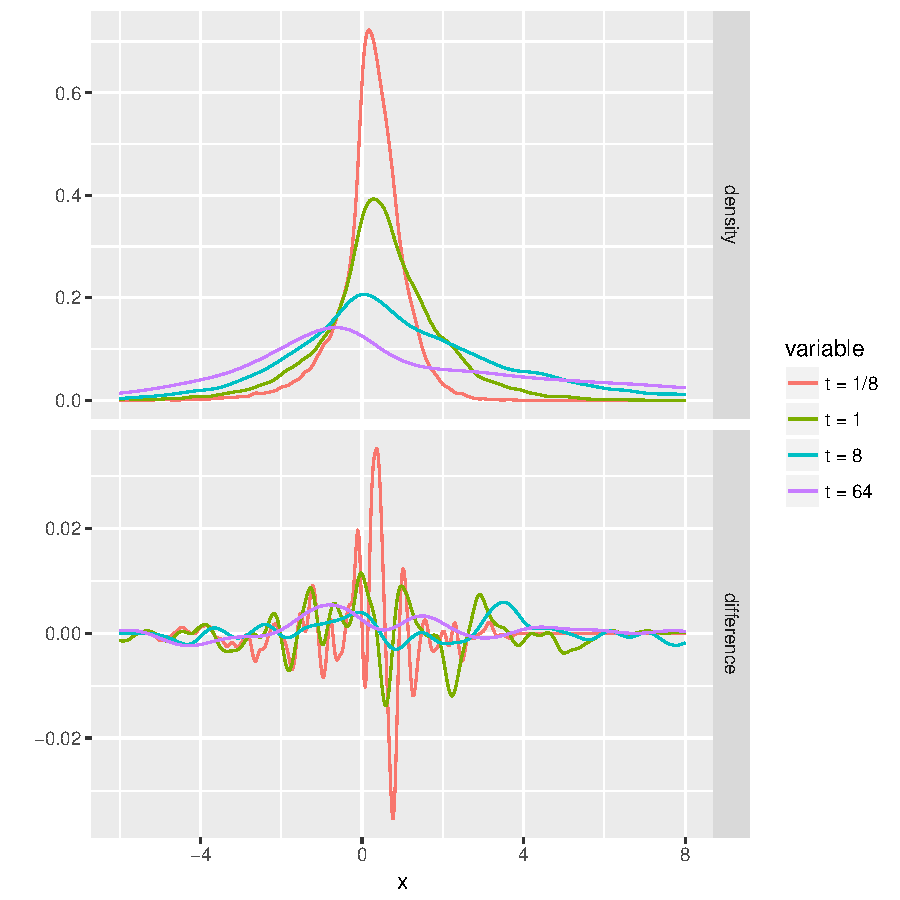
\includegraphics[width = 0.95\textwidth]{densities.pdf}
\caption{Comparison of the dynamics of variable fractional order, at two different time scales $T_0$. For $T_0 = 1$ (left plot), diffusivity and drift are constant and equal to $1$; for $T_0 = 10$, these are equal to $T_0^{-\beta(x)}$. Both dynamics appear equivalent, thus supporting the variable order Fractional Fokker-Planck equation \eqref{eq:FFPE-with-scale}.}
\end{figure}


\section{Conclusion}

In this article, we have employed the theory of stochastic differential equations (SDEs) with
L\'evy noise for the general representation of CTRW limit processes with spatially varying memory kernels.  The theory allows for memory kernels of any variety, 
the only restriction on the type of memory kernel being the L\'evy measure condition \eqref{eq:Levy-condition}.  The memory kernel can then be meaningfully varied in space, as long as certain technical assumptions on the SDE coefficient functions (local linear growth \& local Lipschitz continuity) are maintained.  

Our main motivation was to give a rigorous treatment of CTRW scaling limits and FFPEs with spatially varying fractional order, and hence we have focussed on situations of this type. The discussion surrounding variable tempering and temporal drift parameters we have left for future work.  
%In the case of subdiffusion with spatially varying fractional order, w
Here, we have given a derivation which identifies the unique solutions of variable-order FFPE as probability distributions of CTRW scaling limits. 
Moreover, we have constructed a sequence of CTRW processes which converges to the solution of a variable-order FFPE.  We have used this approach to approximate a solution to a variable-order FFPE via Monte Carlo simulation.

The fractional exponent $\beta$ has traditionally been used to define a global fractional diffusion coefficient, of dimension Length$^2$ / Time$^\beta$.  For spatially varying $\beta(x)$, such a global diffusion coefficient no longer exists.  
Instead, a factor $T_0^{-\beta(x)}$ arises in the variable order FFPE, where $T_0$ corresponds to the applicable unit of time.  We have given a dimensional analysis which shows that the variable order FFPE is dimensionally consistent.  Finally, our simulations confirm that although the drift and diffusivity parameters seemingly depend on the chosen time scale $T_0$ and thus yield different governing FFPEs, the solutions of these different FFPEs are identical and hence that the theory is consistent. 

Currently, there exist few numerical methods for the solution of FFPEs with memory kernels which vary in space, although such FFPEs may well be useful to the physics community, as discussed in the introduction.  The algorithm from \cite{Gill2016} may be extended to the spatially inhomogeneous setting, an idea which we will follow up on in future work. 


\subsection*{Acknowledgements}
Peter Straka was supported by the Australian Research Council via a 
Discovery Early Career Researcher Award (DECRA) DE160101147. 
The author thanks Christopher Angstmann, Gurtek Gill, 
Sergei Fedotov, Bruce Henry, James Nichols and Nickolay Korabel for stimulating discussions which 
significantly improved the presentation of this article. 

\section*{References}

\newcommand{\etalchar}[1]{$^{#1}$}
\begin{thebibliography}{TNMT{\etalchar{+}}04}

\bibitem[ADH13]{Angstmann2013}
Christopher~N Angstmann, I~C Donnelly, and Bruce~I Henry.
\newblock {Continuous Time Random Walks with Reactions Forcing and Trapping}.
\newblock {\em Math. Model. Nat. Phenom.}, 8(2):17--27, apr 2013.

\bibitem[App09]{Applebaum}
D.~Applebaum.
\newblock {\em {L{\'{e}}vy Processes and Stochastic Calculus}}, volume 116 of
  {\em Cambridge Studies in Advanced Mathematics}.
\newblock Cambridge University Press, 2nd edition, may 2009.

\bibitem[Ber99]{Bertoin04}
Jean Bertoin.
\newblock {\em {Subordinators: examples and applications}}, volume 1717 of {\em
  Lecture Notes in Mathematics}.
\newblock Springer Berlin Heidelberg, Berlin, Heidelberg, 1999.

\bibitem[BF05]{Banks2005}
Daniel~S. Banks and C{\'{e}}cile Fradin.
\newblock {Anomalous diffusion of proteins due to molecular crowding.}
\newblock {\em Biophys. J.}, 89(5):2960--71, nov 2005.

\bibitem[BG90]{BG1990}
Jean~Philippe Bouchaud and Antoine Georges.
\newblock {Anomalous diffusion in disordered media: Statistical mechanisms,
  models and physical applications}, nov 1990.

\bibitem[Bil68]{Billingsley1968}
P.~Billingsley.
\newblock {\em {Convergence of Probability Measures}}.
\newblock Wiley Series in Probability and Statistics. John Wiley \& Sons Inc,
  New York, second edition, jan 1968.

\bibitem[BM01]{Baeumer2001}
Boris Baeumer and Mark~M Meerschaert.
\newblock {Stochastic solutions for fractional Cauchy problems}.
\newblock {\em Fract. Calc. Appl. Anal.}, 4(4):481--500, 2001.

\bibitem[BMK00]{BMK00}
Eli Barkai, Ralf Metzler, and Joseph Klafter.
\newblock {From continuous time random walks to the fractional Fokker-Planck
  equation}.
\newblock {\em Phys. Rev. E}, 61(1):132--138, jan 2000.

\bibitem[BS16]{BaeumerStraka16}
Boris Baeumer and Peter Straka.
\newblock {Fokker–Planck and Kolmogorov backward equations for continuous
  time random walk scaling limits}.
\newblock {\em Proc. Am. Math. Soc.}, 145(1):399--412, jul 2016.

\bibitem[CGS05]{Chechkin2005a}
Aleksei~V Chechkin, R.~Gorenflo, and Igor~M Sokolov.
\newblock {Fractional diffusion in inhomogeneous media}.
\newblock {\em J. Phys. A. Math. Gen.}, 38(42):L679--L684, oct 2005.

\bibitem[CLAT10]{Chen2010}
Chang-Ming Chen, F.~Liu, V.~Anh, and I.~Turner.
\newblock {Numerical Schemes with High Spatial Accuracy for a Variable-Order
  Anomalous Subdiffusion Equation}.
\newblock {\em SIAM J. Sci. Comput.}, 32(4):1740--1760, jan 2010.

\bibitem[FF12]{Fedotov2012}
Sergei Fedotov and Steven Falconer.
\newblock {Subdiffusive master equation with space-dependent anomalous exponent
  and structural instability}.
\newblock {\em Phys. Rev. E}, 85(3):031132, mar 2012.

\bibitem[HKRU11]{Hahn11}
Marjorie~G Hahn, Kei Kobayashi, J.~Ryvkina, and Sabir Umarov.
\newblock {On time-changed Gaussian processes and their associated
  Fokker-Planck-Kolmogorov equations}.
\newblock {\em Electron. Commun. Probab.}, 16:150--164, 2011.

\bibitem[HLS10]{HLS10PRL}
Bruce~I Henry, T.~A.~M. Langlands, and Peter Straka.
\newblock {Fractional Fokker-Planck Equations for Subdiffusion with Space- and
  Time-Dependent Forces}.
\newblock {\em Phys. Rev. Lett.}, 105(17):170602, oct 2010.

\bibitem[Kal02]{Kallenberg}
O.~Kallenberg.
\newblock {\em {Foundations of Modern Probability}}.
\newblock Probability and its Applications (New York). Springer, New York, jan
  2002.

\bibitem[KB10]{Korabel2010}
Nickolay Korabel and Eli Barkai.
\newblock {Paradoxes of subdiffusive infiltration in disordered systems}.
\newblock {\em Phys. Rev. Lett.}, 104(17):1--4, 2010.

\bibitem[LHW08]{Langlands2008d}
T.~A.~M. Langlands, Bruce~I Henry, and Susan~L Wearne.
\newblock {Anomalous subdiffusion with multispecies linear reaction dynamics}.
\newblock {\em Phys. Rev. E}, 77(2):021111, feb 2008.

\bibitem[MK00]{Metzler2000}
Ralf Metzler and Joseph Klafter.
\newblock {The random walk's guide to anomalous diffusion: a fractional
  dynamics approach}.
\newblock {\em Phys. Rep.}, 339(1):1--77, dec 2000.

\bibitem[RVD{\etalchar{+}}13]{Regner2013}
Benjamin~M. Regner, Dejan Vu{\v{c}}ini{\'{c}}, Cristina Domnisoru, Thomas~M.
  Bartol, Martin~W. Hetzer, Daniel~M. Tartakovsky, and Terrence~J. Sejnowski.
\newblock {Anomalous diffusion of single particles in cytoplasm}.
\newblock {\em Biophys. J.}, 104(8):1652--1660, 2013.

\bibitem[SCC09]{Sun2009}
HongGuang Sun, Wen Chen, and YangQuan Chen.
\newblock {Variable-order fractional differential operators in anomalous
  diffusion modeling}.
\newblock {\em Phys. A Stat. Mech. its Appl.}, 388(21):4586--4592, nov 2009.

\bibitem[SF15]{StrakaFedotov14}
Peter Straka and Sergei Fedotov.
\newblock {Transport equations for subdiffusion with nonlinear particle
  interaction}.
\newblock {\em J. Theor. Biol.}, 366:71--83, feb 2015.

\bibitem[SH11]{StrakaHenry}
Peter Straka and Bruce~I Henry.
\newblock {Lagging and leading coupled continuous time random walks, renewal
  times and their joint limits}.
\newblock {\em Stoch. Process. their Appl.}, 121(2):324--336, feb 2011.

\bibitem[SM75]{Scher1975}
H.~Scher and E.W.~W Montroll.
\newblock {Anomalous transit-time dispersion in amorphous solids}.
\newblock {\em Phys. Rev. B}, 1975.

\bibitem[SS11]{Stickler2011}
B.~A. Stickler and E.~Schachinger.
\newblock {Continuous time anomalous diffusion in a composite medium}.
\newblock {\em Phys. Rev. E - Stat. Nonlinear, Soft Matter Phys.}, 84(2):1--9,
  2011.

\bibitem[Str17]{var-order-MC}
Peter Straka.
\newblock {Supporting Documentation}, 2017.

\bibitem[SWDA06]{Santamaria2006a}
Fidel Santamaria, Stefan Wils, Erik {De Schutter}, and George~J. Augustine.
\newblock {Anomalous diffusion in Purkinje cell dendrites caused by spines.}
\newblock {\em Neuron}, 52(4):635--48, nov 2006.

\bibitem[TNMT{\etalchar{+}}04]{TMT04}
Iva~Marija Toli{\'{c}}-N{\o}rrelykke, Emilia-Laura Munteanu, Genevieve Thon,
  Lene Oddershede, and Kirstine Berg-S{\o}rensen.
\newblock {Anomalous Diffusion in Living Yeast Cells}.
\newblock {\em Phys. Rev. Lett.}, 93(7):078102, aug 2004.

\bibitem[Tsu92]{Tsuchiya1992}
Masaaki Tsuchiya.
\newblock {L{\'{e}}vy measure with generalized polar decomposition and the
  associated SDE with jumps}.
\newblock {\em Stochastics}, 1129(March 2013):37--41, 1992.

\bibitem[WGR{\etalchar{+}}04]{Wong04}
I.~Y. Wong, M.~L. Gardel, D.~R. Reichman, Eric~R. Weeks, M.~T. Valentine, A.~R.
  Bausch, and D.~A. Weitz.
\newblock {Anomalous Diffusion Probes Microstructure Dynamics of Entangled
  F-Actin Networks}.
\newblock {\em Phys. Rev. Lett.}, 92(17):30--33, 2004.

\bibitem[Whi01]{Whitt2010}
Ward Whitt.
\newblock {\em {Stochastic-Process Limits: An Introduction to
  Stochastic-Process Limits and their Application to Queues}}.
\newblock Springer, New York, 1st edition, nov 2001.

\bibitem[WM08]{Weron2008}
A.~Weron and Marcin Magdziarz.
\newblock {Modeling of subdiffusion in space-time-dependent force fields beyond
  the fractional Fokker-Planck equation}.
\newblock {\em Phys. Rev. E}, 77(3):1--6, mar 2008.

\end{thebibliography}


\appendix

\section{Appendix}

\subsection{Lipschitz and growth conditions on the coefficients} 
\label{subsec:Lip-gro}
After truncation\footnote{Truncation of jumps has no effect on the existence and 
uniqueness of solutions to Stochastic Differential Equations \cite{Applebaum}.} 
at a number $l > 0$, the variable tempered stable L\'evy 
measure 
\eqref{eq:varying-tempered-stable-levy-measure}
has the same form as the function $g$ in Equation (3.1) of 
\cite{Tsuchiya1992}.  
We note that we may ignore $t$ in their notation (our $u$), since we only 
consider Langevin processes with dynamics that are homogeneous in $u$.
We may also drop $\theta$ in their notation, as our L\'evy noise occurs only 
in the one direction $(0,1)$. 
Then identifying $n(x;\rho) \equiv \exp(\theta(x) w)$, 
$\alpha(x) \equiv \beta(x)$, $\beta(x) \equiv 0$, 
we have $g(x;d\rho) \equiv \nu(w|x)\,dw$. 
The condition $\mathcal L_x([0,\infty), R^d, S, (0,l])$ on $n$, $\alpha$ and 
$\beta$ is satisfied if we assume that $\theta(x)$ and $\beta(x)$ are 
continuously differentiable with bounded derivative. 
If $\theta(x)$ and $\beta(x)$ are also bounded, then all four sub-conditions of 
Condition (II) are easily seen to be satisfied.  
Hence (s. top of page 111) part (ii) of Condition (I) is satisfied. 
Part (i) of Condition (I) is trivially fulfilled since 
$y(x; \rho) = \rho \equiv w$ is the identity function. 
Hence Theorem 2.1 applies, which means that $F(w|x)$ satisfies the Lipschitz 
and growth conditions from Theorem 1.1. 
Since we assume that the remaining coefficients are bounded and differentiable 
with bounded derivative, they also satisfy the Lipschitz and growth conditions, 
and hence the Langevin equations \eqref{eq:SDEY}--\eqref{eq:SDEZ} have a unique 
solution $(Y_u, Z_u)$.


\subsection{Proof of Theorem \ref{theorem1}}

Assume that conditions \eqref{eq:cond1}--\eqref{eq:cond4} all hold. 
Split the domain of integration in \eqref{eq:jump-process-generator} into a local part $L = \{(y,w): |y| \le \varepsilon, \, 0 < w \le \varepsilon\}$ and its complement $L^\complement$. On $L$, we do a Taylor expansion and calculate
\begin{align*}
&c \iint\limits_L [f(x+y, s+w) - f(x,w)] K^{(c)}(y,w|x,s)\,dy\,dw
\\
= &\iint\limits_L \left[y f_x(x,s)
+ w f_s(x,s)
+ \frac{1}{2} y^2 f_{xx}(x,s) 
+ yw f_{xs}(x,s) 
+ w^2 f_{ss}(x,s)
+ o(|y|^2 + |y||w| + |w|^2)\right]
\\
& c K^{(c)}(y,w | x,s) \,dy\,dw
\\
= &f_x(x,s) \iint\limits_L y \,cK^{(c)}(y,w|x,s)\,dy\,dw
+ f_s(x,s) \iint\limits_L w \,cK^{(c)}(y,w|x,s)\,dy\,dw
\\
+ &f_{xx}(x,s) \iint\limits_L y^2 \,cK^{(c)}(y,w|x,s)\,dy\,dw
+ f_{xs}(x,s) \iint\limits_L yw \,cK^{(c)}(y,w|x,s)\,dy\,dw
\\
+ &f_{ss}(x,s) \iint\limits_L w^2 \,cK^{(c)}(y,w|x,s)\,dy\,dw
+ o(1)
\end{align*}
where $o(1)$ is a term that tends to $0$ as $\varepsilon \downarrow 0$. 
For the $yw$-term, we find 
\begin{align*}
\left|\iint\limits_L yw \,cK^{(c)}(y,w|x,s)\,dy\,dw \right|
\le \iint\limits_L |y|w \,cK^{(c)}(y,w|x,s)\,dy\,dw
\\
\le \varepsilon \iint\limits_L w \,cK^{(c)}(y,w|x,s)\,dy\,dw
\to \varepsilon [d(x) + o(1)],
\end{align*}
and the same bound holds for the $w^2$-term. 
We add the above and the integral over the complement $L^\complement$ and let $c \to \infty$, to get
\begin{align*}
f_x(x,s) b(x,s) + o(1) + f_s(x,s) d(x) + o(1) + f_{xx}(x,s) a(x,s) + o(1) 
+ 2\varepsilon [d(x) + o(1)]
\\
+ \iint\limits_{L^\complement} [f(x, s+w) - f(x,s)] \nu(w|x)\,dw.
\end{align*}
As $\varepsilon$ was arbitrary to begin with, we let $\varepsilon \downarrow 0$, 
and the above equals $\mathcal A f(x,s)$. 


\subsection{Calculation for Example \ref{example}}
\label{subsec:calc-for-example}

First, we note that 
\begin{align}
  \overline \nu(w|x) \sim w^{-\beta(x)} / \Gamma(1-\beta(x)), 
  \quad w \downarrow 0, 
\end{align}
and thus the inverse function ${\overline \nu}^{-1}(c|x)$ of 
$z \mapsto \overline \nu(z|x)$ satisfies
\begin{align}
  \overline \nu(z | x) \le c
  \Leftrightarrow z \ge {\overline \nu}^{-1}(c|x)
  \sim (\Gamma(1-\beta(x))c)^{-1/\beta(x)},
\end{align}
Hence from the definition \eqref{eq:def-psi} of $\overline \psi^{(c)}(w|x)$, 
\begin{align}
\label{eq:psi-c}
  c \psi^{(c)}(w|x) = \begin{cases}
  \nu(w | x) & \text{ if } w > C(x,c) 
  := {\overline \nu}^{-1}(c|x) + d(x)/c, 
  \\
  0 & \text{ if } 0 < w \le C(x,c). 
  \end{cases}
\end{align}
Since $C(x,c) \downarrow 0$ as $c \to \infty$, for any $w > 0$
\begin{align} \label{eq:non-local-psi}
c \psi^{(c)}(w|x) \to \nu(w|x),
\quad 
  c \overline \psi^{(c)}(w|x) \to \overline \nu(w|x), \quad c \to \infty. 
\end{align}

We also note that $\psi^{(c)}(w|x)$ is a probability density on the positive 
numbers.  Due to \eqref{eq:psi-c}, for any $w > 0$, and large enough $c$,
\begin{align}
  \psi^{(c)}(w|x) = \nu(w|x) / c \to 0, \quad c \to \infty. 
\end{align}  
Hence as $c \to \infty$, the probability mass of the density 
$\psi^{(c)}(w|x)$ must get concentrated near $0$, i.e.\ 
\begin{align} \label{eq:to-delta}
  \int_0^\infty f(w) \psi^{(c)}(w|x) \to f(0)
\end{align}
for any bounded continuous $f$.

Finally, for any $\varepsilon > 0$,
\begin{align}
\label{eq:local-psi}
\begin{split}
  c \int_0^\varepsilon w \psi^{(c)}(w|x) \,dw
  &= c \int_{C(x,c)}^\varepsilon w \psi^{(c)}(w|x) \,dw
  \\
  &= -c\left[w\overline \psi^{(c)}(w|x)\right]^\varepsilon_{C(x,c)}
  + c \int_{C(x,c)}^\varepsilon \overline \psi^{(c)}(w|x)\,dw
  \\
  &= -c\varepsilon \overline \psi^{(c)}(\varepsilon|x)
  + c C(x,c) \times 1
  + c \int_{C(x,c)}^\varepsilon \overline \psi^{(c)}(w|x)\,dw
  \\
  &\to \varepsilon \overline\nu(\varepsilon | x)
  + d(x) + \int_0^\varepsilon \overline \nu(w|x)\,dw
  \\
  &= d(x) + \mathcal O(\varepsilon^{1-\beta(x)}).
\end{split}
\end{align}

\end{document}
